\makesection{Physics}

\begin{frame}{Physics Engine}
    \begin{itemize}
        \item Designed to enable real-time physics without compromising performance.
        \item Frame rate and physics rate are decoupled to maintain fluid gameplay.
        \item Key components:
        \begin{itemize}
            \item Collision detection and handling
            \item Rigid body dynamics simulation
        \end{itemize}
    \end{itemize}
\end{frame}

\begin{frame}{Collision Detection and Resolution}
    \begin{itemize}
        \item Uses Separating Axis Theorem (SAT) to detect collisions between convex shapes.
        \item Optimizations with swept axis-aligned bounding boxes (AABBs) to enhance accuracy.
        \item Collision depth-based resolution to ensure stability during gameplay.
    \end{itemize}
    \centering
    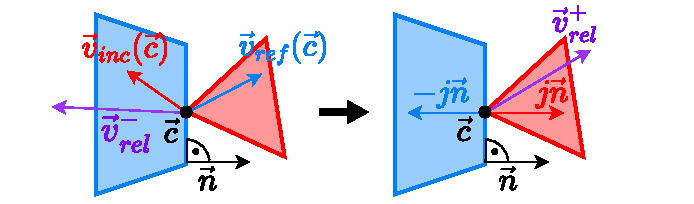
\includegraphics[width=0.6\textwidth]{../figures/physics/resolution.pdf} % Insert collision detection diagram
\end{frame}

\begin{frame}{Performance Considerations}
    \begin{itemize}
        \item Performance optimizations for handling large numbers of entities.
        \item Sub-stepping for fast-moving objects to enhance collision accuracy.
        \item Effective garbage collection for entities and terrain that leave the active area.
    \end{itemize}
\end{frame}